\documentclass[aspectratio=169]{beamer}

\usepackage[ngerman]{babel}
\usepackage[T1]{fontenc}
\usepackage[utf8]{inputenc}
\usetheme{metropolis}
\setbeamertemplate{navigation symbols}{}

\begin{document}

\title{Digital Rights Management}
\subtitle{Encrypted Media Extensions}
\author{Patrick Bucher}
\date{2. Juni 2017}
\maketitle

\begin{frame}
\frametitle{Ablauf}
\tableofcontents
\end{frame}

\section{DRM: Digital Rights Management}
\begin{frame}
\frametitle{Was ist DRM?}
\begin{itemize}
    \item{«Gesamtheit der Strategien und Maßnahmen zur Kontrolle der Nutzung digitaler Medien» (Duden)}
    \item{«Digital \textit{Restriction} Management» (Free Software Foundation)}
\end{itemize}
\end{frame}

\subsection{Einsatzgebiete}
\begin{frame}
\frametitle{Wo wird DRM eingesetzt?}
\begin{itemize}
    \item{physische Medien (CD, DVD, BluRay): Kopieren verhindern}
    \item{eBook-Plattformen (Adobe Digital Editions, Amazon Kindle): Leserechte verwalten}
    \item{Hardware-Schnittstellen (DVI, HDMI): unautorisiertes Abspielen verhindern}
\end{itemize}
\end{frame}

\section{EME: Encrypted Media Extensions}

\subsection{Motivation}
\begin{frame}
\frametitle{Motivation}
\begin{itemize}
    \item{HTML5: Spezifikation des \texttt{<video>}-Elements}
    \item{Problem: HTML5 sieht keine DRM-Mechanismen vor}
    \item{Ziel: Ablösung von Plugins wie Adobe Flash, Microsoft Silverlight etc.}
    \item{Lösungsvorschlag: W3C-Recommendation \textit{Encrypted Media Extensions}}
\end{itemize}
\end{frame}

\subsection{Status}
\begin{frame}
\frametitle{Status}
\begin{itemize}
    \item{W3C: \textit{Proposed Recommendation}}
    \item{Implementierungen: Chrome, Firefox, Safari, Edge und Internet Explorer}
    \item{Beispiel: Netflix auf Chromebooks}
\end{itemize}
\end{frame}

\subsection{Komponenten}
\begin{frame}
\frametitle{Komponenten}
\begin{itemize}
    \item{\textit{License Server}: Ablage der Lizenzschlüssel}
    \item{\textit{Web Application}: Seite mit DRM-geschützten Videos}
    \item{\textit{Content Decryption Module} (CDM): Entschlüsselung geschützter Videos}
\end{itemize}
\end{frame}

\subsection{Ablauf}
\begin{frame}
\frametitle{Ablauf}
\begin{figure}
    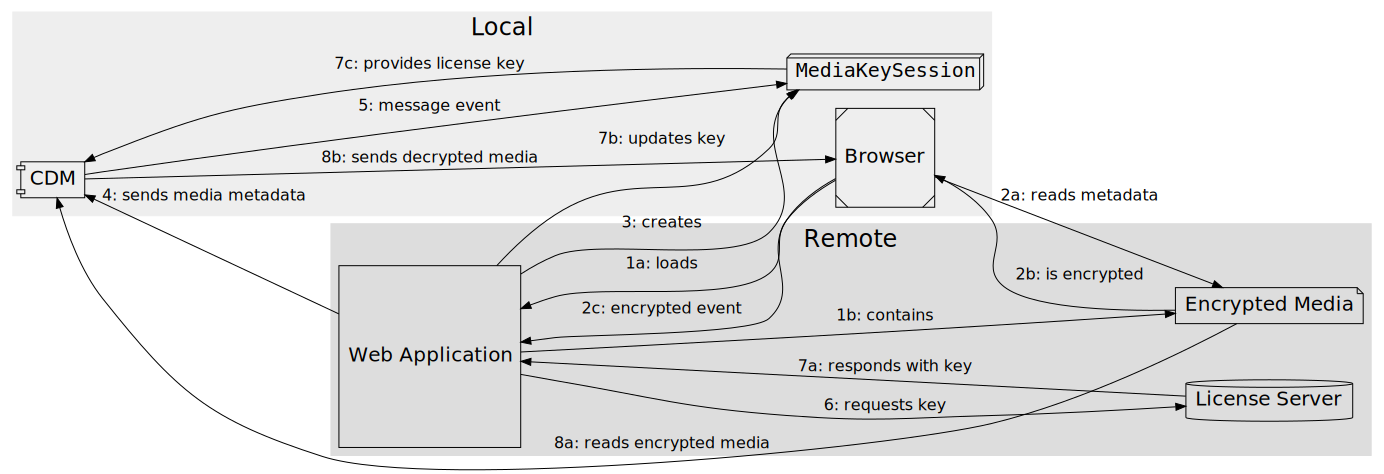
\includegraphics[width=1.0\textwidth]{eme-clustered.png}
    \caption{Das Abspielen eines EME-geschützten Videos}
    \label{fig:EME}
\end{figure}
\end{frame}

\subsection{Kritik}
\begin{frame}
\frametitle{Kritik}
\begin{itemize}
    \item{«Open Web»: Videoanbieter haben die Kontrolle mittels proprietären CDM
        \begin{itemize}
            \item{Beispiel: Netflix 4k-Videos nur auf neuesten Intel «Kaby Lake»-Prozessoren, Windows 10 und Edge-Browser}
        \end{itemize}
    }
    \item{Open Source: Integration geschlossener CDM in offene Browser}
    \item{Sicherheit: Reverse-Engineering von Kopierschutzmechanismen verboten (DMCA)}
\end{itemize}
Meine Meinung: die \textit{Encrypted Media Extensions} laufen der Grundidee des offenen Webs zuwider.
\end{frame}

\begin{frame}
\frametitle{Fragen?}
\end{frame}

\end{document}
